\documentclass{article}
\usepackage[utf8]{inputenc}
\usepackage{bm}
\usepackage{amsmath}
\usepackage{amssymb}
\usepackage{tikz}

\usepackage{geometry}
 \geometry{
 a4paper,
 left=20mm,
 right=20mm,
 top=20mm,
 bottom=20mm
}

\usepackage[math]{cellspace}
\cellspacetoplimit 3pt
\cellspacebottomlimit 3pt
\setlength{\arraycolsep}{4pt}

\makeatletter \g@addto@macro\@floatboxreset\centering \makeatother
    
\newcommand{\norm}[1]{\left\lVert#1\right\rVert}

\title{Gradients and Computational Graph}
\author{Aditya Chopra}
\date{October 2021}

\begin{document}

\maketitle

\section{Computational Graph}

\begin{figure}[!h]
    \centering
    
    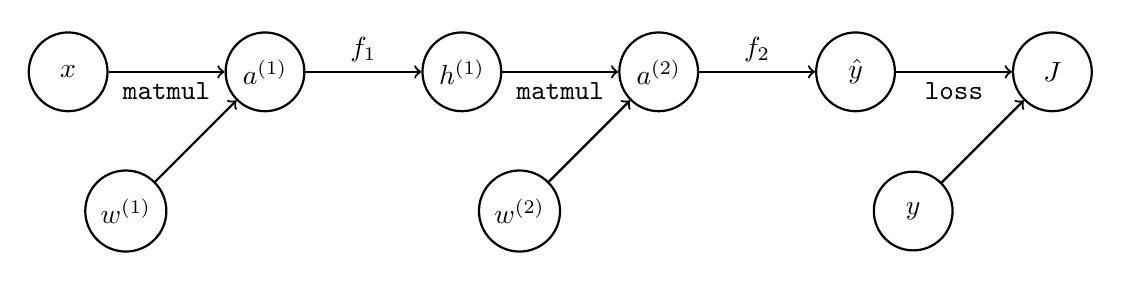
\begin{tikzpicture}[node distance={25mm}, thick, main/.style = {draw, circle, minimum size=10mm}]
        
        \node[main] (1) {$x$};
        \node[main] (2) [right of=1]{$a^{(1)}$};
        \node[main] (3) [below left of=2]{$w^{(1)}$};
        \node[main] (4) [right of=2]{$h^{(1)}$};
        \node[main] (5) [right of=4]{$a^{(2)}$};
        \node[main] (6) [below left of=5]{$w^{(2)}$};
        \node[main] (7) [right of=5]{$\hat y$};
        \node[main] (8) [right of=7]{$J$};
        \node[main] (9) [below left of=8]{$y$};
        
        \draw[->] (1) -- node[midway, below] {\texttt{matmul}} (2);
        \draw[->] (3) -- (2);
        \draw[->] (2) -- node[midway, above] {$f_1$} (4);
        \draw[->] (4) -- node[midway, below] {\texttt{matmul}} (5);
        \draw[->] (6) -- (5);
        \draw[->] (5) -- node[midway, above] {$f_2$} (7);
        \draw[->] (7) -- node[midway, below] {\texttt{loss}}(8);
        \draw[->] (9) -- (8);
        
        
        
    \end{tikzpicture}

    \caption[2 Layer DNN]{Reference Computational Graph for 2 Layer DNN}
\end{figure}


\section{Forward Propagation}

\subsection{Shapes}

\begin{align*}
    x & \in  \mathbb{R}^D \\ 
    w^{(1)} & \in  \mathbb{R}^{D \times M} \\ 
    w^{(2)} & \in  \mathbb{R}^{M \times K}\\
    y & \in  \mathbb{R}^K \\
\end{align*}

\subsection{Equations}

\begin{align}
    a^{(1)} &= w^{(1)T} \cdot x & \left[  a^{(1)} \in \mathbb{R}^M \right] \\
    h^{(1)} &= f_1(a^{(1)}) & \left[ h^{(1)} \in \mathbb{R}^M \right]
\end{align}

\begin{align}
    a^{(2)} &= w^{(2)T} \cdot h^{(1)} & \left[  a^{(2)} \in \mathbb{R}^K \right] \\
    \hat y  &= f_2(a^{(2)}) & \left[  \hat y \in \mathbb{R}^K \right]
\end{align}

\begin{align}
    J = \mathcal{L}(y, \hat  y)
\end{align}

\pagebreak


\section{Backward Propagation}

\subsection{Gradient of a scalar with respect to a vector}
    
\begin{align}
    x \in \mathbb{R}^m \quad y \in \mathbb{R}^n \quad z \in \mathbb{R}
\end{align}

Abstraction 1:

\begin{align}
    \left( \nabla_xz \right)_i = \frac{\partial z}{\partial x_i}
\end{align}

Chain Rule:

\begin{align}
    \nabla_{x}z &= \left( \frac{\partial y}{\partial x} \right)^T  \nabla_{y}z
\end{align}

Where, $\frac{\partial y}{\partial x}$ is the Jacobian Matrix and

\begin{align}
    \frac{\partial y}{\partial x} \in \mathbb{R}^{n \times m}
\end{align}


\subsection{Gradient of a scalar with respect to a tensor}

$X$ and $Y$ are tensors in multiple dimensions.

Abstraction 1:

\begin{align}
    \left( \nabla_Xz \right)_i = \frac{\partial z}{\partial X_i}
\end{align}

Chain Rule:

\begin{align}
    \nabla_{X}z &= \sum_j \left( \nabla_{X}Y_j \right)\frac{\partial z}{\partial Y_j}
\end{align}



\subsection{Equations}

% \begin{align}
%     \nabla_{^{()}}J &= \left( \frac{\partial}{\partial} \right)^T \nabla_{}J
% \end{align}

\begin{align}
    \nabla_{\hat y}J &= \nabla_{\hat y}\mathcal{L}(\hat y, y) &\left[ \nabla_{\hat y}J \in \mathbb{R}^{K} \right] \\ 
    \intertext{}
    \nabla_{a^{(2)}}J &= \left( \frac{\partial \hat y}{\partial a^{(2)}} \right)^T \nabla_{\hat y}J & \left[ \frac{\partial \hat y}{\partial a^{(2)}} \in \mathbb{R}^{K \times K}, \quad \nabla_{a^{(2)}}J
     \in \mathbb{R}^{K} \right] \\
    \intertext{}
    \nabla_{w^{(2)}}J &= \sum_j \left( \nabla{w^{(2)}} Y_j \right) \frac{\partial J }{\partial Y_j } & \left[  \right]\\
    \intertext{}
\end{align}

\end{document}